\documentclass[11pt]{article}
\usepackage[utf8]{inputenc}
\usepackage[margin=0.8in]{geometry}
\usepackage{amsfonts, amsmath}
\usepackage{tikz}
\usepackage[nobreak=false]{mdframed}
\usepackage{pgf}
\usepackage{enumitem}
\usepackage{mathtools}
\usepackage{bbm}
\usepackage{bm}
\usepackage{graphicx}
\usepackage{url}
\usepackage{enumitem}
\usepackage{amsthm,amssymb}
\usepackage{minted}
\setlength\parindent{0pt}
\newcommand{\solution}{\subsection*{Solution:}}

\begin{document}

\title{EE127/227A Homework 1}
\author{Vighnesh Iyer}
\date{\today}
\maketitle

\subsection*{Exercise 1 (CVX Installation)}

For Python users:
Install the package CVXOPT and run the tutorial on Linear Program solvers: \url{http://cvxopt.org/examples/tutorial/lp.html}

For MATLAB users: Install CVX and make sure you can run the least squares code: \url{http://cvxr.com/cvx/doc/quickstart.html}

\begin{solution}
I'm using CVXOPT. From Wikipedia, linear programs can be expressed in canonical form:
\begin{align}
    \text{Minimize  } &\bm{c}^T \bm{x} \nonumber \\
    \text{subject to  } &A\bm{x} \leq \bm{b} \nonumber \\
    \text{and  } &\bm{x} \geq 0 \nonumber
\end{align}

In the tutorial, the following problem is given:
\begin{align}
    \text{Minimize  } &2 x_1 + x_2 \nonumber \\
    \text{subject to  } &-x_1 + x_2 \leq 1 \nonumber \\
    &x_1 + x_2 \geq 2 \nonumber \\
    &x_2 \geq 0 \nonumber \\
    &x_1 - 2x_2 \leq 4 \nonumber
\end{align}

So we can write down the matrices by pattern matching:
\begin{align}
    c &= \begin{bmatrix}
         2 \\ 1
         \end{bmatrix} \nonumber \\
    b &= \begin{bmatrix}
         1 \\ -2 \\ 0 \\ 4
         \end{bmatrix} \nonumber \\
    A &= \begin{bmatrix}
         -1 & 1 \\ -1 & -1 \\ 0 & -1 \\ 1 & -2
         \end{bmatrix} \nonumber
\end{align}

Then use cvxopt to solve
\begin{minted}{python}
from cvxopt import matrix, solvers
A = matrix([ [-1.0, -1.0, 0.0, 1.0], [1.0, -1.0, -1.0, -2.0] ])
b = matrix([ 1.0, -2.0, 0.0, 4.0 ])
c = matrix([ 2.0, 1.0 ])
sol=solvers.lp(c,A,b)
print(sol['x'])
# [ 5.00e-01]
# [ 1.50e+00]
\end{minted}

\end{solution}

\newpage
\subsection*{Exercise 2 (About general optimization)}

In this exercise, we test your understanding of the general framework of optimization and its language. We consider an optimization problem in standard form:
\begin{align*}
    p^* = \min_{x \in \mathbb{R}^n} \: f_0(x) ~:~ f_i(x) \le 0, \;\; i=1,\ldots,m.
\end{align*}
In the following we denote by ${\cal X}$ the feasible set. For the following statements, provide a proof or counter-example.

\begin{enumerate}
    \item Any optimization problem can be expressed as one with a linear objective.

    \item Any optimization problem can be expressed as one without any constraints.

    \item Any optimization problem can be recast as a linear program, provided one allows for an infinite number of constraints.

    \item If one inequality is strict at the optimum, then we can remove it from the original problem and obtain the same solution.

    \item If the problem involves the minimization over more than one variable, say $y$ and $x$, then we can exchange the minimization order without altering the optimal value:
    \begin{align*}
    \min_x\min_y \: F_0(x,y) = \min_y\min_x \: F_0(x,y)
    \end{align*}

    \item If the problem involves the minimization of an objective function of the form
    \begin{align*}
    f_0(x) = \max_y \: F_0(x,y),
    \end{align*}
    then $p^* \ge d^*$, where
    \begin{align*}
    p^* &:= \min_{x} \max_y F_0(x, y) \\
    d^* &:= \max_y \: \min_{x} \: F_0(x,y).
    \end{align*}
    {\em Hint:} consider the function $y \rightarrow \min_{x'} \: F_0(x',y)$ and a similar function of $x$.
\end{enumerate}

\begin{solution}
\begin{enumerate}
\item Yes, this is true. Move the non-linear objective function to the constraint list as such:
\begin{align*}
    p^* &= \min_{y} y \\
    \text{subject to } &f_i(\bm{x}) \leq 0, i = 1,\dots,m \\
    \text{and } &f_0(\bm{x}) \leq y \\
    \text{for } &\bm{x} \in \mathbb{R}^n
\end{align*}

\item Yes, this is true. Move the constraints to the original objective function to increase the cost when the constraint isn't met.
\begin{align*}
    p_{new}^* = \min_{x \in \mathbb{R}^n} f_0(x) + \sum_{i=1}^m \max(f_i(x),0)
\end{align*}

\item Yes, this is true. First, from subsection 1, we can always transform an optimization problem into one with a linear objective. Then, to express any (potentially non-linear) constraint as a set of infinite linear constraints, form a bijection $\mathbb{R}^n \rightarrow \mathbb{R}$ (e.g. decimal place interleaving in the interval (0, 1)), evaluate the constraint on all points in $\mathbb{R}^n$ and for each point create a row in $A$ and entry in $b$ that indicates whether the constraint is satisfied or not.
%This may be true, but I don't know of a good way to prove it yet. alright, now i don't think this is true because how can you express a constraint like cos(x) \leq 0 into a linear system (even if infinite). ok I again think this is true, but I need to be able to formally put any non-linear constraint in terms of an infinite number of linear constraints.

\item A counter-example exists. An inequality being strict at the optimum means that it is \textbf{not} satisfied at the optimum, but just barely so.
\begin{align*}
    x^* &= \min_{x} x^2 : x > 0 \\
    \text{without strict constraint } x^* &= 0 \\
    \text{with strict constraint } x^* &= \text{infinitely close to 0, but not 0}
\end{align*}

\item Yes, this is true. A minimization over 1 variable must consider all possible values of the other variable, so the order of minimization cannot matter. If minimization over 1 variable can't be performed without knowledge of the other variable, then the order of minimization cannot matter, and in the case where minimization over 1 variable allows for elimination of that variable the same can be said.

\item \textbf{TODO TODO TODO}
\end{enumerate}
\end{solution}

\newpage
\subsection*{Exercise 3 (1D Convolution)}

A 1D convolutional filter takes an input sequence $x = (x_t)_{t \in \mathbb{Z}}$ and a finite sequence $h = (h_t)_{t \in [1, m]}$ and produces an output sequence according to the rule

\[y_t = h_1x_t + h_2x_{t-1} + ... + h_mx_{t-m+1},  t \in \mathbb{Z}\]

This operation is mathematically denoted $y = h * x$ and called a convolution. Now consider a sequence $x$ such that $x_t = 0$ for $t < 1$ and $t > n$. We will from now refer to \emph{infinite-dimensional} vector $x$ as the \emph{finite-dimensional} vector $(x_1, ..., x_n)$.

\begin{enumerate}
    \item Show that the output sequence $(y_t)_{t \in \mathbb{Z}}$ is zero outside a band. In particular, you will show that $y_t = 0$ for $t \leq a$ and $t > b$ for $(a, b)$ that you will determine as a function of $n$ and $m$. The output sequence can therefore be represented as a $(b-a)$-dimensional vector that we will note $y = (y_{a+1}, ..., y_{b})$.

    \item Express the relationship between the output vector $y$ and $x$ as $y = T(h) \cdot x$, with $T(h)$ a matrix of shape $(b-a, n)$. What structure does that matrix have?

    \item We consider two $n$-th order polynomials $p$, $q$:
    \begin{align*}
        p(s) &= p_0s^0 + p_1s^1 + ... + p_ns^n \\
        q(s) &= q_0s^0 + q_1s^1 + ... + q_ns^n.
    \end{align*}
    Express the product of the polynomials in terms of vectors of coefficients of $p$, $q$, and powers of $s$, and a certain Toeplitz matrix, which you will determine.

    \item A given $T$-vector $r$ gives the daily rainfall in some region over a period of $T$ days. The vector $h$ gives the daily height of a river in the region (above its normal height). By careful modeling of water flow, or by fitting a model to past data, it is found that these vectors are (approximately) related by convolution: $h=g*r$, where $g= (0.1,0.4,0.5,0.2)$. How  many days  after a  one day heavy rainfall is the river height most affected? And, how many days does it takes for the river height to return to the normal height once the rain stops?
\end{enumerate}

\begin{solution}
\begin{enumerate}
\item We can write $y_t$ as:
\begin{align*}
    y_t &= \begin{cases}
        0 & t \leq 0 \\
        \sum_{i=1}^{m} h_i x_{t-i-1} & t > 0 \land t \leq n + m - 1 \\
        0 & t > n + m - 1
    \end{cases} \\
    a &= 0 \\
    b &= n + m - 1
\end{align*}
When $t \leq 0$, all the terms of $y_t$ become 0. After that point, every value of $y_t$ can be non-zero until the $x_t$ vector has 'passed' the convolution taps.

\item The matrix is a Toeplitz matrix (each descending diagonal from left to right is constant).
\begin{align*}
    \begin{bmatrix}
        y_1 \\ y_2 \\ \vdots \\ y_{b-a}
    \end{bmatrix}
    =
    \begin{bmatrix}
        h_1 & 0 & \dots & 0 & 0 \\
        h_2 & h_1 & \dots & 0 & 0 \\
        \vdots & \vdots & \vdots & h_1 & 0 \\
        h_{m} & h_{m-1} & \dots & h_2 & h_1 \\
        0 & h_m & \dots & h_{m-2} & h_{m-1} \\
        0 & 0 & \dots & h_{m-1} & h_{m-2} \\
        0 & 0 & 0 & h_{m} & h_{m-1} \\
        0 & 0 & 0 & 0 & h_m
    \end{bmatrix}
    \begin{bmatrix}
        x_1 \\ x_2 \\ \vdots \\ x_n
    \end{bmatrix}
\end{align*}

\item The product of $p(s)$ and $q(s)$ can be given in the form $(\mathbf{T} \mathbf{p})^T \mathbf{s}$, where $\mathbf{T}$ is the constructed Toeplitz matrix, $\mathbf{p}$ is a vector composed of polynomial coefficients (i.e. $p_0, p_1, \dots, p_n$) , and $\mathbf{s}$ is a vector of powers of $s$ (i.e. $s^0, s^1, \dots, s^n$).

    \begin{align*}
    T =
    \begin{bmatrix}
        p_0 & 0 & \dots & 0 & 0 \\
        p_1 & p_0 & \dots & 0 & 0 \\
        \vdots & \vdots & \vdots & p_1 & 0 \\
        p_{n} & p_{n-1} & \dots & p_1 & p_0 \\
        0 & p_n & \dots & p_{n-2} & p_{n-1} \\
        0 & 0 & \dots & p_{n-1} & p_{n-2} \\
        0 & 0 & 0 & p_{n} & p_{n-1} \\
        0 & 0 & 0 & 0 & p_n
    \end{bmatrix}
    \end{align*}
\item It takes 2 days after heavy rainfall for the river height to become maximal because there are 2 taps of 'delay' before the heavy rainfall day lands on the 0.5 multiplier. Similarly, it takes 3 days after heavy rainfall (counting the day that the rain stops) for the river height to go back to 'normal' because there are only 4 coefficients in $g$ before the heavy rainfall day no longer affects $h$.
\end{enumerate}
\end{solution}

\newpage
\subsection*{Exercise 4 (Norm and angles)}

\begin{enumerate}
    \item Let $x,y\in\mathbb{R}^{n}$ be two unit-norm vectors, that is, such that $\|x\|_2 = \|y\|_2=1$. Show that the vectors $x-y$ and $x+y$ are orthogonal. Draw on the 2D plane the two vectors and all the necessary shapes to graphically solve the exercise. You may use right angles, circles and straight lines to make your point.

    \item
    Show that the following inequalities hold for any vector $x \in \mathbb{R}^{n}$:
    \begin{align*}
        \frac{1}{\sqrt{n}}\|x\|_2 \leq \|x\|_\infty \leq  \|x\|_2 \leq \|x\|_1 \leq \sqrt{n} \|x\|_2 \le n\|x\|_\infty.
    \end{align*}
    \textit{Hint:} think about using Cauchy-Schwarz's inequality, and instantiate it on the corresponding norms.

    \item Show that for any non-zero vector $x$,
    \begin{align*}
        \text{card}(x) \ge \frac{\|x\|_1^2}{\|x\|_2^2},
    \end{align*}
    where $\text{card}(x)$ is the \emph{cardinality} of the vector $x$, defined as the number of non-zero elements in $x$. Find all vectors $x$ for which the lower bound is attained.
\end{enumerate}

\begin{solution}
\begin{enumerate}
\item
\begin{align*}
    x - y \text{ orthogonal to } x + y &\rightarrow (x-y) \cdot (x+y) = 0 \\
    (x-y)_i &= x_i - y_i \\
    (x+y)_i &= x_i + y_i \\
    (x-y) \cdot (x+y) &= \sum_{i=1}^n (x-y)_i (x+y)_i = \sum_{i=1}^n (x_i-y_i)(x_i+y_i) \\
    &= \sum_{i=1}^n x_i^2 - y_i^2 = \sum_{i=1}^n x_i^2 - \sum_{i=1}^n y_i^2 \\
    &= ||x||_2^2 - ||y||_2^2 = 1 - 1 = 0
\end{align*}
        \begin{figure}[H]
            \centerline{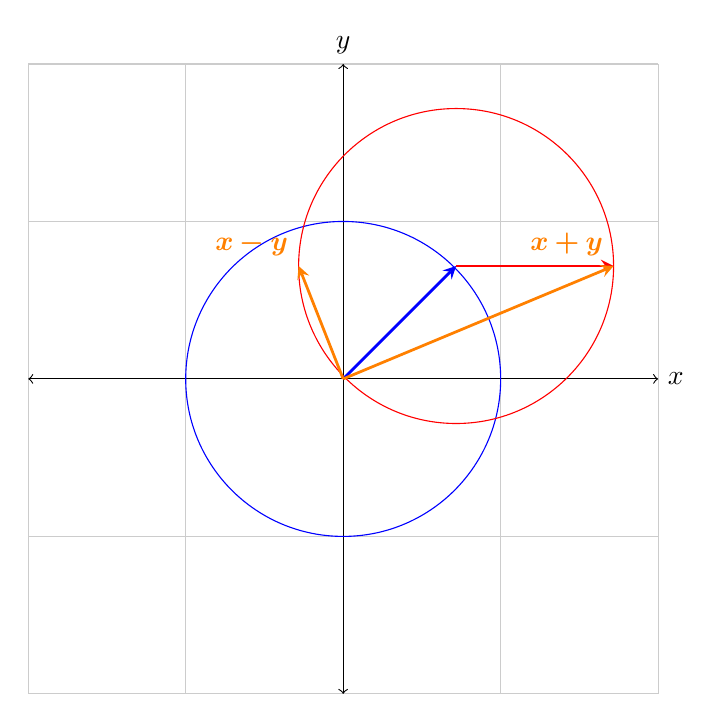
\begin{tikzpicture}[scale=2]
          \draw[thin,gray!40] (-2,-2) grid (2,2);
          \draw[<->] (-2,0)--(2,0) node[right]{$x$};
          \draw[<->] (0,-2)--(0,2) node[above]{$y$};
          \draw[blue] (0,0) circle [radius=1];
          \draw[red] (0.717, 0.717) circle [radius=1];
          \draw[line width=1pt,blue,-stealth](0,0)--(0.717,0.717) node[anchor=north]{$\boldsymbol{}$};
          \draw[line width=1pt,red,-stealth](0.717,0.717)--(1.717,0.717) node[anchor=north east]{$\boldsymbol{}$};
          \draw[line width=1pt,orange,-stealth](0,0)--(1.717,0.717) node[anchor=south east]{$\boldsymbol{x+y}$};
          \draw[line width=1pt,orange,-stealth](0,0)--(-0.283,0.717) node[anchor=south east]{$\boldsymbol{x-y}$};
            \end{tikzpicture}}
        \end{figure}

        The blue circle represents all possible choices of $x$ and the red circle shows all the points to which $x+y$ can extend if $x$ was picked to be $[0.717, 0.717]$. The diagram shows that if $y$ is moved to hit a different point on the red circle, it amounts to a rotation of $x+y$ and $x-y$, but the angle between them stays at 90 deg.

\item Prove the inequalities from left to right
\begin{align*}
    \text{Prove: } \frac{1}{\sqrt{n}} ||x||_2 \leq ||x||_{\infty} \\
    ||x||_2^2 = \sum_{i=1}^n x_i^2 &\leq n \cdot \max_{i=1,\dots,n} x_i^2 n \cdot \max_{i=1,\dots,n} |x_i|^2 = n ||x||_{\infty}^2 \\
    \rightarrow ||x||_2^2 &\leq n ||x||_{\infty}^2 \\
    \rightarrow \frac{1}{\sqrt{n}} ||x||_2 \leq ||x||_{\infty}
\end{align*}

\begin{align*}
    \text{Prove: } \|x\|_{\infty} &\leq \|x\|_2 \\
    \|x\|_{\infty} &= \max_{i=i,\dots,n} |x_i| = \max_{i=1,\dots,n} \sqrt{|x_i|^2} \leq \sqrt{\sum_{i=1}^n |x_i|^2} = \|x\|_2 \\
    \rightarrow \|x\|_{\infty} &\leq \|x\|_x
\end{align*}

\begin{align*}
    \text{Prove: } \|x\|_2 &\leq \|x\|_1 \\
    \text{In general } \sqrt{a_1 + a_2 + \dots + a_n} &\leq \sqrt{a_1} + \sqrt{a_2} + \dots + \sqrt{a_n} \\
    \|x\|_2 = &\sqrt{\sum_{i=1}^n |x_i|^2} \leq \sum_{i=1}^n \sqrt{|x_i|^2} = \|x\|_1 \\
    \rightarrow \|x\|_2 &\leq \|x\|_1
\end{align*}

\begin{align*}
    \text{Prove: } \|x\|_1 &\leq \sqrt{n} \|x\|_2 \\
    \text{Let: } x &= \begin{bmatrix} |x_1| & |x_2| & \dots & |x_n| \end{bmatrix}^T \\
        y &= \begin{bmatrix} 1 & 1 & \dots & 1 \end{bmatrix}^T \\
    \text{Applying C-S: } |x^T y| &\leq \|x\|_2 \|y\|_2 \\
    | \sum_{i=1}^n |x_i| | &\leq \|x\|_2 \sqrt{n} \\
    \|x\|_1 &\leq \sqrt{n} \|x\|_2
\end{align*}

\begin{align*}
    \text{Prove: } \sqrt{n} \|x\|_2 &\leq n \|x\|_{\infty} \\
    \text{We had shown: } \|x\|_2^2 &\leq n \|x\|_{\infty}^2 \\
    n \|x\|_2^2 &\leq n^2 \|x\|_{\infty}^2 \\
    \sqrt{n} \|x\|_2 &\leq n \|x\|_{\infty}
\end{align*}

\item
    \begin{align*}
        \|x\|_1 &= \sum_{i=1}^n |x_i| \cdot c_i \\
        \text{Let } c_i &= \begin{cases}
            0 & x_i = 0 \\
            1 & \text{otherwise}
        \end{cases} \\
        \text{By C-S } \|x\|_1 &\leq \||x_i|\|_2 \cdot \|c_i\|_2 \\
        &\leq \sqrt{\sum_{i=1}^n |x_i|^2} \sqrt{\sum_{i=1}^n c_i^2} \\
        &\leq \|x\|_2 \cdot \sqrt{card(x)} \\
        \rightarrow \frac{\|x\|_1^2}{\|x\|_2^2} &\leq card(x)
    \end{align*}
\end{enumerate}
\end{solution}

\newpage
\subsection*{Exercise 5 (Comparing text)}

In this exercise, we  use the word-fre\-quen\-cy vector representation of text
 for comparing  text documents. For mathematical modeling of transforming text into vectors, refers to Lecture 2, Slide 6 (Example 1: bag of words).
In this context, similarity between two documents may be measured by means of the angle $\theta$ between the two frequency vectors
representing the documents, the documents being maximally ``different'' when the corresponding frequency vectors are orthogonal.
Consider the following
headlines from the web edition of the New York Times on Dec.\ 7, 2010:

\begin{enumerate}[label=(\alph*)]
    \item Suit Over Targeted Killing in Terror Case Is Dismissed. A federal judge on Tuesday dismissed a lawsuit that sought to block the United States from attempting to kill an American citizen, Anwar Al-Awlaki, who has been accused of aiding Al Qaeda.

    \item In Tax Deal With G.O.P., a Portent for the Next 2 Years. President Obama made clear that he was willing to alienate his liberal base in the interest of compromise. Tax Deal Suggests New Path for Obama. President Obama agreed to a tentative deal to extend the Bush tax cuts, part of a package to keep jobless aid and cut payroll taxes.

    \item Obama Urges China to Check North Koreans. In a frank discussion, President Obama urged China's president to put the North Korean government on a tighter leash after a series of provocations.

    \item Top Test Scores From Shanghai Stun Educators. With China's debut in international standardized testing, Shanghai students have surprised experts by outscoring counterparts in dozens of other countries.
\end{enumerate}

\begin{enumerate}
    \item
    First simplify the text (remove plurals, convert verb to infinite tense, etc.) and then find the frequency vectors   representing the text against the dictionary $V=\{$aid, kill, deal, president, tax, china$\}$.

    \item Compare the four pieces of text by computing the cosine distance (i.e the cosine of the angles) between any pairs of texts.
\end{enumerate}

\begin{solution}
\begin{enumerate}
\item
\begin{align*}
    a = \begin{bmatrix} 1& 2& 0& 0& 0& 0 \end{bmatrix}^T \\
    b = \begin{bmatrix} 1& 0& 3& 2& 4& 0 \end{bmatrix}^T \\
    c = \begin{bmatrix} 0& 0& 0& 2& 0& 2 \end{bmatrix}^T \\
    d = \begin{bmatrix} 0& 0& 0& 0& 0& 1 \end{bmatrix}^T
\end{align*}

\item
\begin{minted}{python}
pairs = [
    (a,a),(a,b),(a,c),(a,d),
    (b,b),(b,c),(b,d),(c,c),(c,d),(d,d)
]
pairs_eng = [
    '(a,a)','(a,b)','(a,c)','(a,d)',
    '(b,b)', '(b,c)','(b,d)','(c,c)','(c,d)','(d,d)'
]
for ((x,y),eng) in zip(pairs,pairs_eng):
    print(eng + ":")
    print(np.dot(x.T, y) / (np.linalg.norm(x,2) * np.linalg.norm(y,2)))
\end{minted}

\begin{minted}{text}
(a,a):
0.9999999999999998
(a,b):
0.0816496580927726
(a,c):
0.0
(a,d):
0.0
(b,b):
1.0
(b,c):
0.2581988897471611
(b,d):
0.0
(c,c):
0.9999999999999998
(c,d):
0.7071067811865475
(d,d):
1.0
\end{minted}
\end{enumerate}
\end{solution}

\newpage
\subsection*{Exercise 6 (Linear functions and projections)}

\begin{enumerate}
    \item Suppose $x$ is an $n$-vector, with $n = 2m - 1$ and $m \geq 1$. We define the middle element value of $x$ as $x_m$. Define $$f(x) = x_m - \frac{1}{n}\sum_{i = 1}^n x_i$$ which is the difference between the middle element value and the average of the coefficients in $x$. Express $f$ in the form $f(x) = a^Tx$, where $a$ is an $n$-vector.

    \item Now let $b$ and $x$ be vectors of $\mathbb{R}^2$ (with $\|b\|_2 = 1$). Draw on the 2-D plane $b$, $x$ and show the value of $b^Tx$ on the graph.
\end{enumerate}

Now we will focus on Senator Voting data. This data provides information about senator vote $x$ and senator political affiliation $y$. We provide you with four different vectors $(a_1, a_2, a_3, a_4)$ precomputed by the EECS127 staff. Each of these vectors can be used to define a linear function $f_a: x \rightarrow a^Tx$.

\begin{enumerate}
    \item[3.] Load the files in \textit{senator.zip}, and let $X$ be the data matrix (with each row a senator, and each column a bill). Center the data matrix $X$ (which is a standard preprocessing step for data analysis) and then compute for each vector $a$ the score of each senator. We provide you with the skeleton code to load the data and visualize the scores in contrast to the affiliation $y$. You will compute such plots using the existing code and explain them.

    \item[4.] Which direction among the vectors $a_1, a_2, a_3, a_4$ do you prefer in order to produce a score that effectively summarizes the affiliation? Justify your answer.
\end{enumerate}

\begin{solution}
\begin{enumerate}
    \item Construct $\mathbf{a}$ as such:
        \begin{align*}
            a = \begin{bmatrix} -\frac{1}{n} & -\frac{1}{n} & \dots & -\frac{1}{n} + 1 & \dots & -\frac{1}{n} & -\frac{1}{n} \end{bmatrix}^T
        \end{align*}
    \item Projection of $x$ onto $b$:
        \begin{figure}[H]
            \centerline{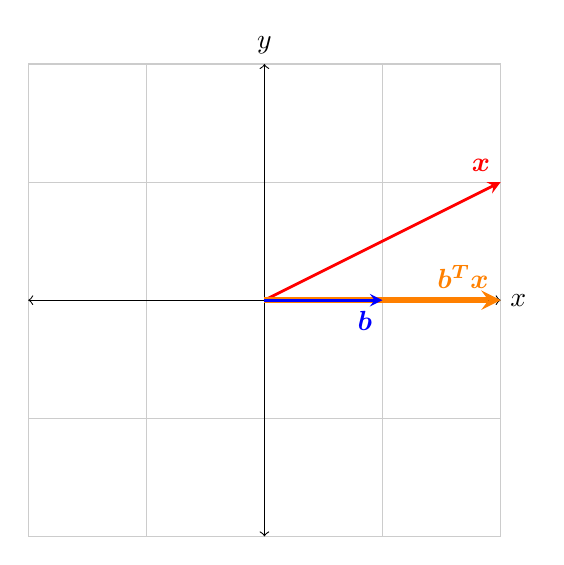
\begin{tikzpicture}[scale=1.5]
          \draw[thin,gray!40] (-2,-2) grid (2,2);
          \draw[<->] (-2,0)--(2,0) node[right]{$x$};
          \draw[<->] (0,-2)--(0,2) node[above]{$y$};
          \draw[line width=1pt,red,-stealth](0,0)--(2,1) node[anchor=south east]{$\boldsymbol{x}$};
          \draw[line width=2pt,orange,-stealth](0,0)--(2,0) node[anchor=south east]{$\boldsymbol{b^Tx}$};
          \draw[line width=1pt,blue,-stealth](0,0)--(1,0) node[anchor=north east]{$\boldsymbol{b}$};
          %\draw[line width=1pt,orange,-stealth](0,0)--(-0.283,0.717) node[anchor=south east]{$\boldsymbol{x-y}$};
            \end{tikzpicture}}
        \end{figure}
    \item To subtract the mean from the data matrix $X$:
    \begin{minted}{python}
    X_bar = np.zeros(X.shape)
    col_means = X.mean(axis=0)
    for col in range(X.shape[1]):
        for row in range(X.shape[0]):
            X_bar[row,col] = X[row,col] - col_means[col]
    print(X_bar)
    \end{minted}
    To compute the senator scores:
    \begin{minted}{python}
    senator_scores = np.dot(a_vectors, X_bar)
    \end{minted}
    \begin{figure}[H]
        \centerline{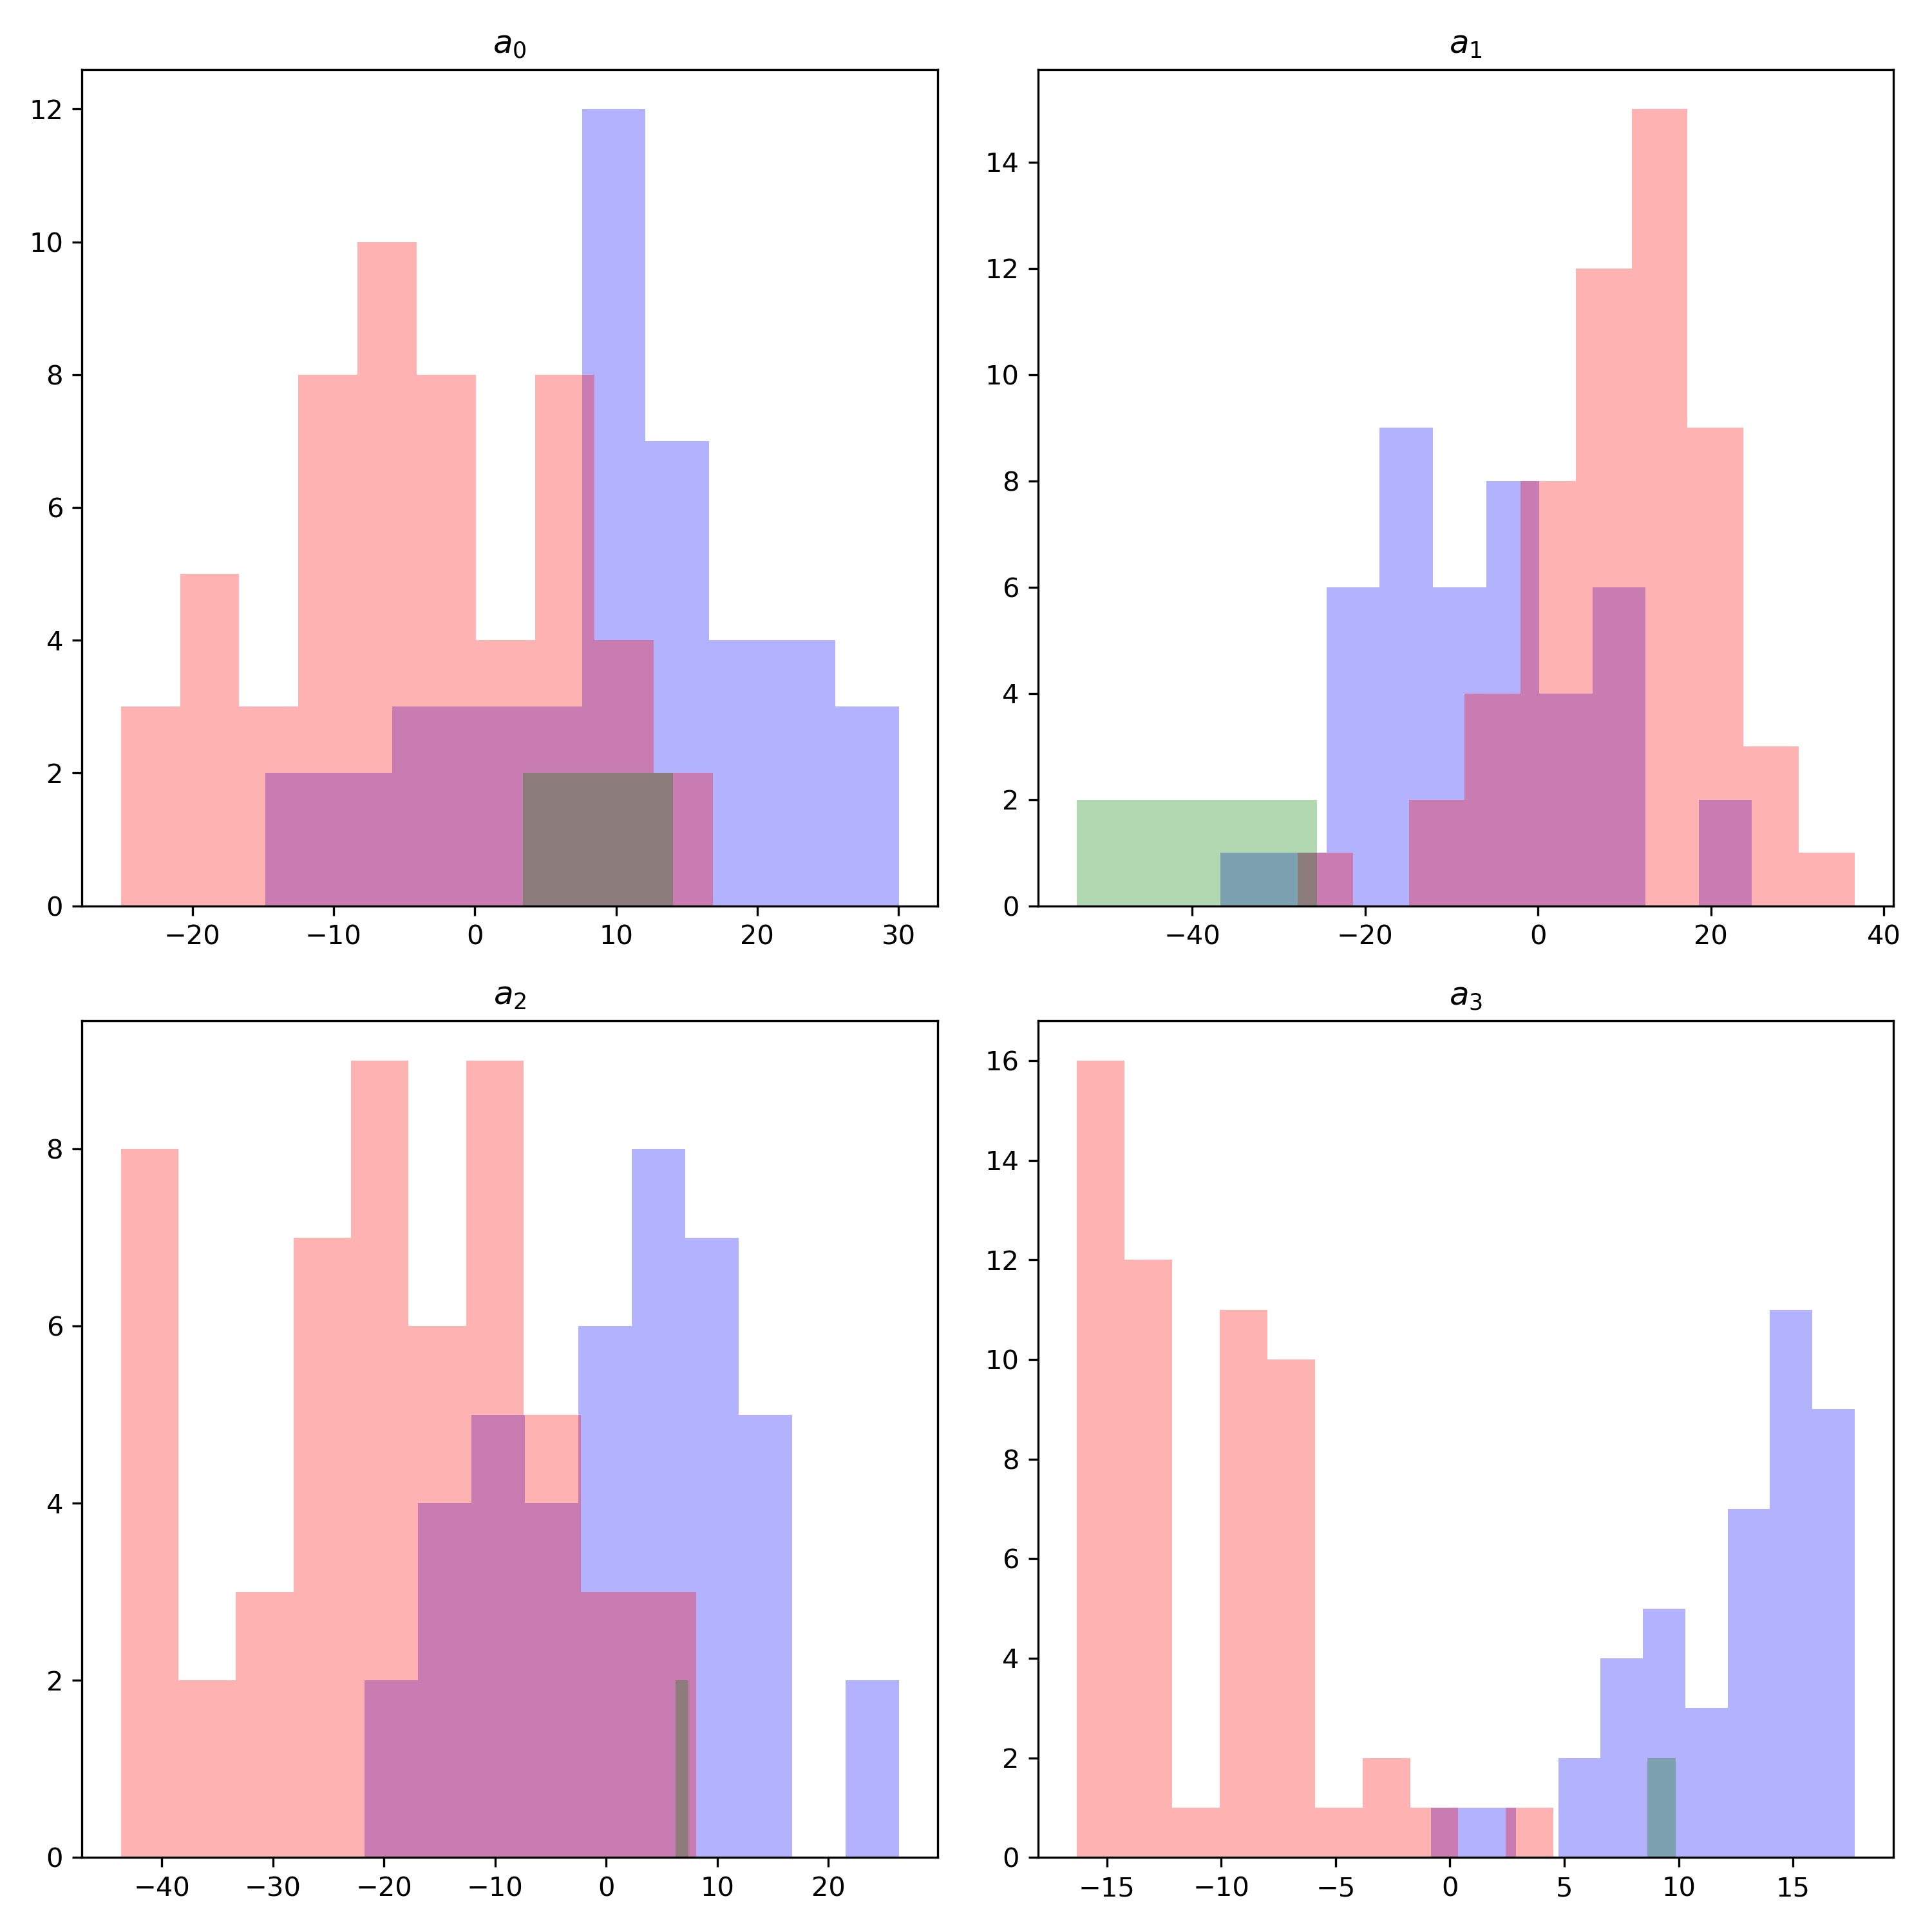
\includegraphics[width=0.6\textwidth]{figs/exercise_6.png}}
    \end{figure}
    \item Direction $a_4$ clearly works the best to separate senators based on affilation. Look at the large score difference between red and blue senators for vector $a_4$ but the large overlap with the other vectors.
\end{enumerate}
\end{solution}

\newpage
\subsection*{Exercise 7 (Customer purchase history matrix)}

A store keeps track of its sales of products from $K$ different
product categories to $N$ customers over some time period, like one month. $K$ might be on the order of 1000 and $N$ might be 100000. The data is stored in an $N \times K$ matrix $C$, with $C_{ij}$ being the total dollar purchases of product $j$ by customer $i$ All the entries of $C$ are non-negative. The matrix $C$ is typically sparse, i.e., many of its entries are zero.

\begin{enumerate}
    \item What is $C \boldsymbol{1}$? ($\boldsymbol{1}$ is a $K$-vector of 1s)

    \item What is $C^T \boldsymbol{1}$? ($\boldsymbol{1}$ is a $N$-vector of 1s)

    \item Give a short matrix-vector expression for the total dollar amount of all purchases, by all customers.

    \item What does it mean if ($CC^T)_{kl} = 0$? Your answer should be simple English.
\end{enumerate}

We are now interested in efficient computations. In our setting, note that the data matrix $C$ is large but very sparse. The number of non zero-valued elements divided by the total number of elements is called the density $d$ of the matrix $C$. Let $w$ in $\mathbb{R}^K$ be a given weighting vector. Assume that we center the rows (removing the average row to every row), obtaining a new row-centered matrix $C_m$.

\begin{enumerate}
    \item[5.] Provide an explanation on how to efficiently compute the matrix vector product $v = C_m w$.

    \item[6.] Mathematically estimate the gain speed of your method vs the naive method (of forming $C_m$ first) as a function of $K$, $N$, and $d$.

    \item[7.] Confirm your findings with an empirical study: we provide you with a matrix $C$ and a vector $w$ in the Jupyter Notebook matrix-vector.ipynb. Using the skeleton code, compare the sparse matrix method against the naive method. Comment on the time improvement and attach your notebook here in pdf format for grading. Let us note that we do not ask the students to create their own sparse matrix functionalities.

    \item[8.] Assume that we add one row (data point). Explain how to efficiently update the resulting vector $v$ accordingly.
\end{enumerate}

\begin{solution}
\begin{enumerate}
    \item $C \mathbf{1}$ returns a vector representing the total purchase amount (in dollars) per customer.
    \item $C^T \mathbf{1}$ returns a vector representing the total purchased amount (in dollars) per product.
    \item $(C \mathbf{1}_K)^T \mathbf{1}_N$ where $\mathbf{1}_x$ is a length $x$ vector of 1s.
    \item If $(C C^T)_{k,l} = 0$ it means customer $k$ and customer $l$ didn't purchase any products in common.
    \item Let $\mathbf{m}$ denote the row average vector, which containes $K$ elements. We can express the first row (sum) of $\mathbf{v} = C_m \mathbf{w}$ as such:
        \begin{align*}
            \mathbf{v}_0 &= (C_{0,0} - m_0) w_0 + (C_{0,1} - m_1) w_1 + \dots + (C_{0,K-1} - m_{K-1}) w_{K-1} \\
            \text{Combining terms: } \mathbf{v}_0 &= (C_{0,0}w_0 + \dots + C_{0,K-1}w_{K-1}) - (m_0 w_0 + \dots + m_{K-1} w_{K-1}) \\
        \end{align*}
        Note that the first term can be formed with $C_{sparse} \cdot \mathbf{w}$ and the second term can be formed with $\mathbf{m} \cdot \mathbf{w}^T$ and they can be subtracted.
    \item The naive method would first perform $N \cdot K$ subtractions to form $C_m$, then $K \cdot N$ multiplications and $(K-1) \cdot N$ additions to form $\mathbf{v}$.

        Total naive: $2 N K$ multiplications and $(K-1) N$ additions.

        The optimized method would perform $K$ multiplications and $K-1$ additions to form $\mathbf{m} \cdot \mathbf{w}^T$. Due to sparsity, the operations used to compute $C_{sparse} \cdot \mathbf{w}$ will be scaled from the naive method by density $d$ to get $K \cdot N \cdot d$ multiplications and $(K-1) \cdot N \cdot d$ additions. Finally, to form $\mathbf{v}$, we need $N$ subtractions.

        Total optimized: $K + KNd$ multiplications and $K-1 + (K-1) N d + N$ add/sub operations.

        Rounding $K-1$ to $K$ and estimating that multiplications have about the same throughput as add or subtract ops:
        \begin{align*}
            \text{Naive ops } &= 3NK \\
            \text{Opt ops } &= 2K + 2KNd + N
        \end{align*}

    \item In this notebook, $N = K = 10000$ and $d = 0.1$, so the $\text{naive ops } = 300000000$, and $\text{opt ops } = 20030000$ for an estimated 15X speedup.

    The naive implementation:
    \begin{minted}{python}
        (C - r_avg) @ w
    \end{minted}
    \begin{minted}{text}
        CPU times: user 487 ms, sys: 211 ms, total: 697 ms
        Wall time: 472 ms
    \end{minted}

    The optimized implementation:
    \begin{minted}{python}
        np.subtract(C_sparse @ w, r_avg @ w)
    \end{minted}
    \begin{minted}{text}
        CPU times: user 27.9 ms, sys: 26.8 ms, total: 54.7 ms
        Wall time: 53 ms
    \end{minted}

    Equivalence Check:
    \begin{minted}{python}
        gold = (C - r_avg) @ w
        opt = np.subtract(C_sparse @ w, r_avg @ w)
        np.allclose(gold, opt) # account for floating-point errors
    \end{minted}
    \begin{minted}{text}
        True
    \end{minted}

    I actually got a 9X speedup, which is close enough. Probably I need to put more weight on the multiplication ops over the add/sub ops.

    \item Adding a new row will change $\mathbf{m}$, the row average vector. Assuming $C_{sparse} \cdot \mathbf{w}$ is cached, just recompute $\mathbf{m} \cdot \mathbf{w}^T$ and subtract to refresh the existing elements of $\mathbf{v}$.

        Then to add a new element to $\mathbf{v}$, take the new row $\mathbf{r}$ on its own and perform $\mathbf{r} \cdot \mathbf{w}$, then subtract $\mathbf{m} \cdot \mathbf{w}^T$ from it.
\end{enumerate}
\end{solution}

\end{document}
